\documentclass[letterpaper,12pt]{article}
\setlength{\headheight}{15pt}
\setlength{\marginparwidth}{0pt}
\setlength{\marginparsep}{0pt} % width of space between body text and margin notes
\setlength{\evensidemargin}{0.125in} % Adds 1/8 in. to binding side of all 
% even-numbered pages when the "twoside" printing option is selected
\setlength{\oddsidemargin}{0.125in} % Adds 1/8 in. to the left of all pages when "oneside" printing is selected, and to the left of all odd-numbered pages when "twoside" printing is selected
\setlength{\textwidth}{6.375in} % assuming US letter paper (8.5 in. x 11 in.) and side margins as above
\raggedbottom
\setlength{\parskip}{\medskipamount}

\usepackage{pgfplots}
\usepackage{amsmath, amsthm, amssymb, fancyhdr, enumitem, tikz}
\pagestyle{fancy}
\lhead{MATH350 --- HW4}
\begin{document}
\begin{enumerate}
    \item There are 5 closed boxes on a table. Three of the boxes have good prizes inside and the
other two don’t. You open boxes one at a time until you find a prize. Let $X$ be the
number of boxes you open.
    \begin{enumerate}[label=(\alph*).]
        \item Find the pmf of $X$.
            \paragraph{Ans:} $X$ may take values $\in [1,3]$. Let $f(X)$ be the pmf of $X$.
            \[ f(X) = \begin{cases}
                \frac{3}{5}& x = 1\\
                \frac{2}{5}\cdot\frac{3}{4}& x = 2 \\
                \frac{2}{5} \cdot \frac{1}{4} \cdot 1 & x = 3 \\
                0 & x > 3
                \end{cases}
            \]
        \item Find $E(X)$.
            \paragraph{Ans:} 
            \begin{equation}
                E(X) = \sum_k k P(X=k)
            \end{equation}
            \paragraph{}Alternate symbol of $E[X] = \mu$
            \paragraph{}Thus
            \begin{align*}
                E(X) &= 1\cdot\frac{2}{5} + 2\bigg(\frac{2}{5}\cdot \frac{3}{4}\bigg) + 3\cdot\bigg(\frac{2}{5} \cdot \frac{1}{4}\bigg)\\
                     &= 1.3
            \end{align*}
        \item Find Var$(X)$.
            \paragraph{Ans:}
            \begin{equation}
                \mathrm{Var}(X) = \sum_k (k-\mu)^2 P(X=k)
            \end{equation}
            \begin{align*}
                \mathrm{Var}(X) &= (1-1.3)^2\cdot\frac{2}{5}+(2-1.3)^2\bigg(\frac{2}{5}\cdot \frac{3}{4}\bigg) + (3-1.3)^2\bigg(\frac{2}{5}\cdot \frac{1}{4}\bigg)\\
                                &= .4720
            \end{align*}
        \item Suppose the good prize inside each of the three boxes is \$100, but each empty box
you open costs you \$100. What is your expected gain or loss in the game? (Hint:
Express the gain or loss as a function of $X$.)
\paragraph{Ans:}
\[ f(X) = \begin{cases}
    100 & x = 1 \\
    0 & x = 2 \\
    -100 & x = 3 \\
    \end{cases}
\]
\begin{align*}
    E[X] &= 100\cdot\frac{3}{5} + 0 -100\cdot\bigg(\frac{2}{5}\cdot\frac{1}{4}\bigg)\\
         &= 50
\end{align*}
    \end{enumerate}
\item Let $X$ be a random variable with density function
    \[ f(x) = \begin{cases}
        \frac{1}{4} & 1 <x<2 \\
        c & 3 < x < 5\\
        0 & \mathrm{otherwise}
        \end{cases}
    \]
    \begin{enumerate}[label=(\alph*).]
        \item Find the value of c.
            \paragraph{Ans:} By the properties of a density function,
            \[
                \int_{-\infty}^{\infty} f(x)\,dx = 1
            \]
            \paragraph{}which is only possible given $c$ is equal to
            \begin{align*}
                c(5-3) &= 1 - \frac{1}{4}(2-1)\\
                2c &= .75\\
                 c &= \frac{3}{8}
            \end{align*}
        \item Find $P(1.5 < X < 4)$
            \paragraph{Ans:}
            \begin{align*}
                P(a < X < b) &= \int_b^a f(x)\,dx\\
                P(1.5 < X < 4) &= \int_{1.5}^4 f(x)\,dx\\
                               &= \int_{1.5}^2 f(x)\,dx + \int_2^3 f(x)\,dx+\int_3^4 f(x)\,dx\\
                               &= \frac{1}{2}(2-1.5) + 0 + \frac{3}{8}(4-3)\\
                               &= .50
            \end{align*}
        \item Find the cdf of $X$.
            \paragraph{Ans:}
            \begin{align*}
                F(s) = P(X\le s) &= \int_{-\infty}^s f(x)\,dx\\
                                 &= \begin{cases}
                                     0 & s < 1 \\
                                     \frac{s-1}{4} & 1 < s < 2 \\
                                     \frac{3}{8}(s-3)+.25 & 3 < s < 5 \\
                                     1 & x > 5 \\
                                     \end{cases}
            \end{align*}
    \end{enumerate}
\item Choose a point $(X,Y )$ uniformly inside the triangle with vertices (0,0), (30,0) and
(30,20).



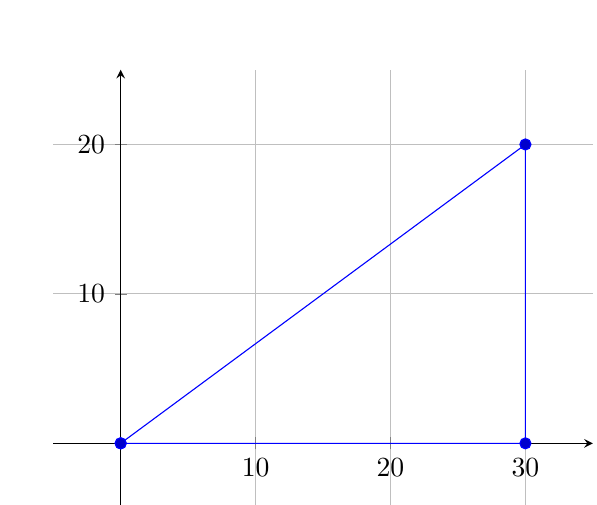
\begin{tikzpicture}
 \pgfplotsset{compat=newest,compat/show suggested version=false}
   \pgfplotsset{filter discard warning=false}
\pgfplotsset{compat=1.7}

\begin{axis}[xmin=-5, xmax=35, ymin=-5, ymax=25, axis x line=middle, axis y line=middle, grid=both]
    \addplot coordinates{(0,0) (30,0) (30,20) (0,0)};
\end{axis}
\end{tikzpicture}
\begin{enumerate}[label=(\alph*).]
    \item Find the cdf of $X$.
        \paragraph{Ans:} The area inside the triangle may be modeled by 
        \begin{align*}
            \int_{0}^{30} \frac{2}{3}x \, dx = 300
        \end{align*}
        \paragraph{}as $X$ may take values $\in [0,30]$.
        \paragraph{}$$P(X \le x) = \frac{1}{300}\int_0^x \frac{2}{3}x\,dx$$
        \paragraph{}Thus, we write the cdf as
        \[ f(x) = \begin{cases}
            0 & x < 0\\
            \frac{1}{300}\cdot \frac{1}{3}x^2 & 0 \le x \le 30\\
            1 & x > 30
            \end{cases}
        \]
    \item Using (a), find the density function of $X$.
        \paragraph{Ans:}
        \[ f_X(x) = \begin{cases}
            0 & x < 0 \\
            \frac{1}{450}x & x \in [0,30] \\
            0 & x > 30
            \end{cases}
        \]
\end{enumerate}
\item Suppose that when you take the bus to school, it arrives after a uniformly distributed
number of hours in the interval [0,1] after you get to the stop. However, if it does not
arrive for 45 minutes, you take an uber. Let $X$ be the number of hours you wait.
\paragraph{}(a). Find the cdf of $X$.
\paragraph{Ans:} The graph of $X$ is as follows.

\vspace{5mm}

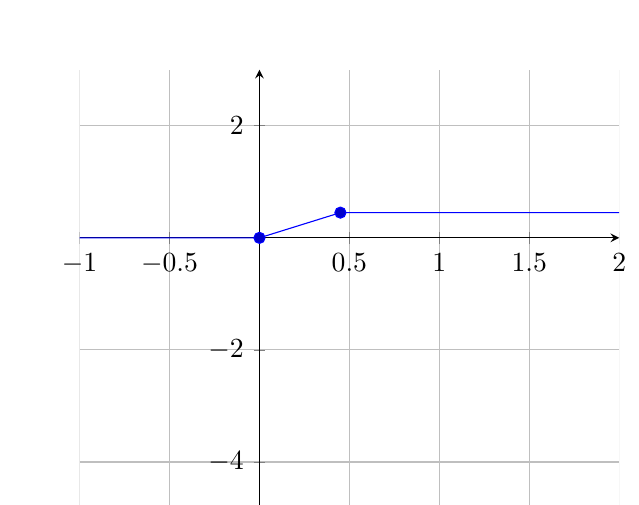
\begin{tikzpicture}
 \pgfplotsset{compat=newest,compat/show suggested version=false}
   \pgfplotsset{filter discard warning=false}
\pgfplotsset{compat=1.7}
\begin{axis}[xmin=-1, xmax=2, ymin=-5, ymax=3, axis x line=middle, axis y line=middle, grid=both]
    \addplot coordinates{(-2,0) (0,0) (.45, .45) (3, .45)};
\end{axis}
\end{tikzpicture}
\paragraph{}Let $Y$ be the time which the bus arrives. $Y \sim U[0,1]$.
\end{enumerate}
\end{document}

